\documentclass{article}
\usepackage{fontspec}
\setsansfont{Helvetica}
\renewcommand{\familydefault}{\sfdefault}
\usepackage{tikz}
\usetikzlibrary{arrows.meta}
\pagestyle{empty}
\definecolor{lookup}{HTML}{2A78D6}
\definecolor{lookuplight}{HTML}{9DC1EC}
\definecolor{write}{HTML}{EB6834}
\definecolor{writelight}{HTML}{F5B597}
\definecolor{ink}{HTML}{0B0B0B}
\definecolor{inktwo}{HTML}{52514E}
\definecolor{gridc}{HTML}{E4E3DF}
\definecolor{axisc}{HTML}{8F8E89}
\definecolor{refc}{HTML}{3D3C39}
\tikzset{
  tick/.style={font=\footnotesize, text=inktwo, inner sep=1.5pt},
  lab/.style={font=\small, text=ink, inner sep=1.5pt},
  note/.style={font=\footnotesize, text=inktwo, inner sep=1.5pt},
  ser/.style={line width=1.4pt, line cap=round, line join=round},
  thin/.style={line width=0.9pt, line cap=round, line join=round},
  ref/.style={line width=0.8pt, draw=refc, dash pattern=on 3pt off 2pt},
}
\begin{document}
\setbox0=\hbox{%
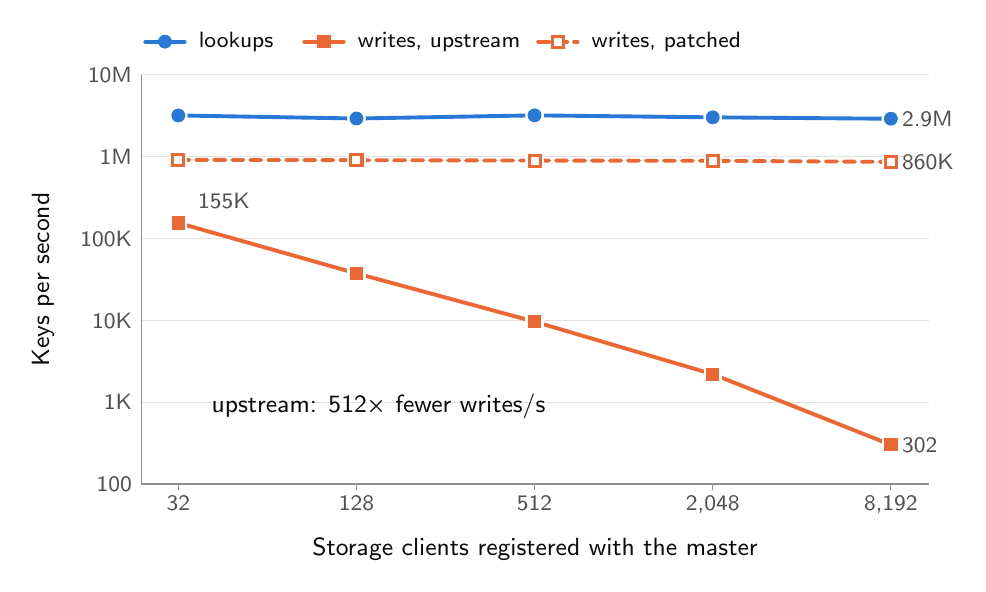
\begin{tikzpicture}[x=1cm,y=1cm]
\draw[draw=gridc, line width=0.4pt] (0.000,0.000) -- (10.000,0.000);
\node[tick, anchor=east] at (-0.060,0.000) {100};
\draw[draw=gridc, line width=0.4pt] (0.000,1.040) -- (10.000,1.040);
\node[tick, anchor=east] at (-0.060,1.040) {1K};
\draw[draw=gridc, line width=0.4pt] (0.000,2.080) -- (10.000,2.080);
\node[tick, anchor=east] at (-0.060,2.080) {10K};
\draw[draw=gridc, line width=0.4pt] (0.000,3.120) -- (10.000,3.120);
\node[tick, anchor=east] at (-0.060,3.120) {100K};
\draw[draw=gridc, line width=0.4pt] (0.000,4.160) -- (10.000,4.160);
\node[tick, anchor=east] at (-0.060,4.160) {1M};
\draw[draw=gridc, line width=0.4pt] (0.000,5.200) -- (10.000,5.200);
\node[tick, anchor=east] at (-0.060,5.200) {10M};
\draw[draw=axisc, line width=0.4pt] (0.469,0.000) -- (0.469,-0.070);
\node[tick, anchor=north] at (0.469,-0.090) {32};
\draw[draw=axisc, line width=0.4pt] (2.732,0.000) -- (2.732,-0.070);
\node[tick, anchor=north] at (2.732,-0.090) {128};
\draw[draw=axisc, line width=0.4pt] (4.994,0.000) -- (4.994,-0.070);
\node[tick, anchor=north] at (4.994,-0.090) {512};
\draw[draw=axisc, line width=0.4pt] (7.257,0.000) -- (7.257,-0.070);
\node[tick, anchor=north] at (7.257,-0.090) {2,048};
\draw[draw=axisc, line width=0.4pt] (9.519,0.000) -- (9.519,-0.070);
\node[tick, anchor=north] at (9.519,-0.090) {8,192};
\draw[draw=axisc, line width=0.5pt] (0.000,5.200) -- (0.000,0.000) -- (10.000,0.000);
\draw[ser, draw=lookup] (0.469,4.683) -- (2.732,4.644) -- (4.994,4.684) -- (7.257,4.659) -- (9.519,4.641);
\draw[ser, draw=write, dash pattern=on 4pt off 2.5pt] (0.469,4.119) -- (2.732,4.115) -- (4.994,4.110) -- (7.257,4.107) -- (9.519,4.093);
\draw[ser, draw=write] (0.469,3.318) -- (2.732,2.677) -- (4.994,2.064) -- (7.257,1.397) -- (9.519,0.500);
\fill[white] (0.469,4.683) circle (3.4pt);
\fill[lookup] (0.469,4.683) circle (2.5pt);
\fill[white] (2.732,4.644) circle (3.4pt);
\fill[lookup] (2.732,4.644) circle (2.5pt);
\fill[white] (4.994,4.684) circle (3.4pt);
\fill[lookup] (4.994,4.684) circle (2.5pt);
\fill[white] (7.257,4.659) circle (3.4pt);
\fill[lookup] (7.257,4.659) circle (2.5pt);
\fill[white] (9.519,4.641) circle (3.4pt);
\fill[lookup] (9.519,4.641) circle (2.5pt);
\fill[white] (0.469,4.119) +(-3.3pt,-3.3pt) rectangle +(3.3pt,3.3pt);
\filldraw[fill=white, draw=write, line width=1.1pt] (0.469,4.119) +(-2.0pt,-2.0pt) rectangle +(2.0pt,2.0pt);
\fill[white] (2.732,4.115) +(-3.3pt,-3.3pt) rectangle +(3.3pt,3.3pt);
\filldraw[fill=white, draw=write, line width=1.1pt] (2.732,4.115) +(-2.0pt,-2.0pt) rectangle +(2.0pt,2.0pt);
\fill[white] (4.994,4.110) +(-3.3pt,-3.3pt) rectangle +(3.3pt,3.3pt);
\filldraw[fill=white, draw=write, line width=1.1pt] (4.994,4.110) +(-2.0pt,-2.0pt) rectangle +(2.0pt,2.0pt);
\fill[white] (7.257,4.107) +(-3.3pt,-3.3pt) rectangle +(3.3pt,3.3pt);
\filldraw[fill=white, draw=write, line width=1.1pt] (7.257,4.107) +(-2.0pt,-2.0pt) rectangle +(2.0pt,2.0pt);
\fill[white] (9.519,4.093) +(-3.3pt,-3.3pt) rectangle +(3.3pt,3.3pt);
\filldraw[fill=white, draw=write, line width=1.1pt] (9.519,4.093) +(-2.0pt,-2.0pt) rectangle +(2.0pt,2.0pt);
\fill[white] (0.469,3.318) +(-3.3pt,-3.3pt) rectangle +(3.3pt,3.3pt);
\fill[write] (0.469,3.318) +(-2.4pt,-2.4pt) rectangle +(2.4pt,2.4pt);
\fill[white] (2.732,2.677) +(-3.3pt,-3.3pt) rectangle +(3.3pt,3.3pt);
\fill[write] (2.732,2.677) +(-2.4pt,-2.4pt) rectangle +(2.4pt,2.4pt);
\fill[white] (4.994,2.064) +(-3.3pt,-3.3pt) rectangle +(3.3pt,3.3pt);
\fill[write] (4.994,2.064) +(-2.4pt,-2.4pt) rectangle +(2.4pt,2.4pt);
\fill[white] (7.257,1.397) +(-3.3pt,-3.3pt) rectangle +(3.3pt,3.3pt);
\fill[write] (7.257,1.397) +(-2.4pt,-2.4pt) rectangle +(2.4pt,2.4pt);
\fill[white] (9.519,0.500) +(-3.3pt,-3.3pt) rectangle +(3.3pt,3.3pt);
\fill[write] (9.519,0.500) +(-2.4pt,-2.4pt) rectangle +(2.4pt,2.4pt);
\node[note, anchor=south west] at (0.662,3.436) {155K};
\node[note, anchor=west] at (9.519,0.500) {\;302};
\node[note, anchor=west] at (9.519,4.093) {\;860K};
\node[note, anchor=west] at (9.519,4.641) {\;2.9M};
\node[lab, anchor=west] at (0.834,0.992) {upstream: 512× fewer writes/s};
\node[lab, anchor=north] at (5.000,-0.620) {Storage clients registered with the master};
\node[lab, rotate=90, anchor=south] at (-1.050,2.600) {Keys per second};
\draw[ser, draw=lookup] (0.050,5.620) -- (0.550,5.620);
\fill[lookup] (0.300,5.620) circle (2.5pt);
\node[note, anchor=west, text=ink] at (0.670,5.620) {lookups};
\draw[ser, draw=write] (2.070,5.620) -- (2.570,5.620);
\fill[write] (2.320,5.620) +(-2.4pt,-2.4pt) rectangle +(2.4pt,2.4pt);
\node[note, anchor=west, text=ink] at (2.690,5.620) {writes, upstream};
\draw[ser, draw=write, dash pattern=on 4pt off 2.5pt] (5.040,5.620) -- (5.540,5.620);
\filldraw[fill=white, draw=write, line width=1.1pt] (5.290,5.620) +(-2.0pt,-2.0pt) rectangle +(2.0pt,2.0pt);
\node[note, anchor=west, text=ink] at (5.660,5.620) {writes, patched};
\end{tikzpicture}}%
\pdfvariable horigin=0pt
\pdfvariable vorigin=0pt
\pagewidth=\dimexpr\wd0+8pt\relax
\pageheight=\dimexpr\ht0+\dp0+8pt\relax
\shipout\vbox{\kern4pt\hbox{\kern4pt\box0\kern4pt}\kern4pt}
\end{document}
